\documentclass[../main.tex]{subfiles}

\addbibresource{\subfix{../references.bib}}

\begin{document}

\ifSubfilesClassLoaded{%
    \setcounter{chapter}{2}%
    \begin{refsection}
}{}

\chapter{Lexical Analysis dan Regular Expression}
\label{chap:lexical-analysis}

\begin{subcpmk}
  \item \textbf{Sub-CPMK 2.1:} Membuat regular expression untuk token spesifik bahasa
  \item \textbf{Sub-CPMK 2.2:} Mengimplementasikan NFA dan DFA untuk token recognition
\end{subcpmk}

% ============================================================
% MATERI POKOK
% ============================================================
\section{Pengenalan Lexical Analysis}

\subsection{Peran Lexical Analyzer}

\compiler{Lexical Analysis} (atau \compiler{Lexer/Scanner}) adalah tahap pertama dalam kompilasi yang bertugas membaca aliran karakter dari program sumber dan mengelompokkannya ke dalam unit-unit bermakna yang disebut \textit{token} \cite{aoyama2024lexical, opengenus2024lexer}.

\begin{itemize}
  \item Menghapus whitespace dan komentar.
  \item Melaporkan lexical error.
\end{itemize}

\subsection{Alur Teoretis Lexical Analysis}

Sebagai landasan untuk memahami lexical analysis, kita perlu mempelajari teori formal yang mendasarinya. Alur ini menunjukkan bahwa lexical analysis dalam kompilator modern menggunakan teori \textit{formal language}, khususnya \textit{regular languages}.

\begin{figure}[!htbp]
    \centering
    \adjustbox{max width=0.85\textwidth,center}{%
    \begin{tikzpicture}[
        box/.style={rectangle, draw=blue!50, fill=blue!10, text width=1.8cm, text centered, minimum height=0.8cm, rounded corners, font=\footnotesize, inner sep=4pt, align=center},
        arrow/.style={->, >=stealth, thick},
        label/.style={font=\tiny, above, align=center},
        node distance=1.8cm
    ]
    \node[box] (regex) {Regular\\Expression};
    \node[box, right=of regex] (nfa) {$\epsilon$-NFA};
    \node[box, right=of nfa] (dfa) {DFA};
    \node[box, right=of dfa] (impl) {Scanner};
    
    \draw[arrow] (regex) -- node[label] {Thompson} (nfa);
    \draw[arrow] (nfa) -- node[label] {Subset\\Const.} (dfa);
    \draw[arrow] (dfa) -- node[label] {Code\\Gen.} (impl);
    \end{tikzpicture}%
    }
    \caption{Alur konversi dari regular expression ke implementasi scanner}
    \label{fig:lexical-theory-overview}
\end{figure}

\subsection{Token dan Lexeme}

\begin{itemize}
  \item \textbf{Token}: Kategori unit leksikal (misal: \keyword{IDENTIFIER}, \keyword{KEYWORD}).
  \item \textbf{Lexeme}: String aktual yang mewakili token (misal: \code{x}, \code{if}).
  \item \textbf{Attribute Value}: Informasi tambahan (misal: nilai literal, entri tabel simbol).
\end{itemize}

\section{Regular Expression}

\subsection{Definisi dan Operasi Dasar}

Regular expression (regex) adalah notasi formal untuk mendeskripsikan pola string dalam suatu \textbf{regular language}. Operasi dasar meliputi:

\begin{table}[h]
\centering
\begin{tabular}{|l|l|l|}
\hline
\textbf{Operasi} & \textbf{Simbol} & \textbf{Contoh} \\
\hline
Karakter & $a$ & string "a" \\
Alternasi & $|$ & $a|b$ (a atau b) \\
Konkatenasi & $ab$ & string "ab" \\
Kleene Star & $*$ & $a^*$ (0 atau lebih) \\
Positive Plus & $+$ & $a^+$ (1 atau lebih) \\
Optional & $?$ & $a?$ (0 atau 1) \\
\hline
\end{tabular}
\caption{Operator dasar Regular Expression}
\end{table}

\subsection{Implementasi Leksikal dengan Regex}

Dalam pembangunan kompilator, setiap elemen leksikal (token) didefinisikan dengan regex guna menjamin kepastian pola:
\begin{itemize}
  \item \textbf{Identifier}: \texttt{[a-zA-Z\_][a-zA-Z0-9\_]*}
  \item \textbf{Integer}: \texttt{[0-9]+}
  \item \textbf{Float}: \texttt{[0-9]+\textbackslash.[0-9]+([eE][+-]?[0-9]+)?}
  \item \textbf{String Literal}: \texttt{"([\textasciicircum"\\]|\textbackslash\textbackslash.)*"}
\end{itemize}

\subsection{Sifat Regular Language}
Bahasa reguler dapat dikenali secara efisien menggunakan finite automata dan tertutup terhadap operasi gabungan, pengulangan, serta penyambungan, namun tidak dapat mendeskripsikan struktur \textit{nested} mendalam.

\section{Finite Automata}

Finite Automata (FA) adalah mesin abstrak yang membaca string input dan memutuskan apakah string tersebut diterima (\textit{accepted}) atau ditolak (\textit{rejected}). FA adalah "mesin" yang menjalankan aturan Regular Expression.

\subsection{NFA: The Parallel Multi-verse}
\compiler{Nondeterministic Finite Automata (NFA)} memiliki kemampuan "magis" untuk berada di beberapa state sekaligus. Jika ada dua transisi keluar dengan label yang sama (atau transisi $\epsilon$), NFA seolah-olah membelah diri dan menelusuri semua jalur yang mungkin secara paralel. Jika salah satu "kloningan" mesin ini berhasil mencapai state akhir, maka input diterima.

\begin{itemize}
    \item \textbf{Fleksibilitas}: Sangat mudah dibentuk langsung dari Regular Expression (misal: a|b langsung menjadi cabang).
    \item \textbf{Biaya}: Sulit diimplementasikan di komputer nyata karena komputer bekerja secara deterministik (serial). Simulasi NFA membutuhkan pelacakan himpunan state aktif yang kompleks.
\end{itemize}

\subsection{DFA: The Realistic Machine}
\compiler{Deterministic Finite Automata (DFA)} adalah mesin yang realistis. Untuk setiap input dan state saat ini, hanya ada \textbf{tepat satu} transisi ke state berikutnya. Tidak ada ambiguitas, tidak ada "tebakan".

\begin{itemize}
    \item \textbf{Efisiensi}: Eksekusi DFA sangat cepat, linear terhadap panjang input ($O(n)$). Lexer komersial selalu menggunakan DFA (atau simulasi DFA) di balik layar.
    \item \textbf{Ukuran}: Jumlah state DFA bisa meledak secara eksponensial dibandingkan NFA asalnya, namun dalam praktik kompilator, ukurannya biasanya masih wajar.
\end{itemize}

\begin{figure}[!htbp]
    \centering
    \adjustbox{max width=1.0\textwidth,center}{%
    \begin{tikzpicture}[
        state/.style={circle, draw=blue!50, fill=blue!10, minimum size=0.6cm, font=\tiny},
        accept/.style={circle, draw=green!50, fill=green!10, minimum size=0.6cm, font=\tiny, double},
        start/.style={circle, draw=red!50, fill=red!10, minimum size=0.6cm, font=\tiny},
        arrow/.style={->, >=stealth, thick},
        node distance=1.2cm
    ]
    \node[start] (nq0) at (0,0) {$q_0$};
    \node[accept] (nq1) at (2,0) {$q_1$};
    \draw[arrow] (nq0) -- node[above, font=\tiny] {a} (nq1);
    \draw[arrow] (nq1) to[loop above] node[above, font=\tiny] {a} (nq1); % Loop on q1
    \node[below=0.4cm of nq0] {DFA untuk $a+$ (menerima "a", "aa", ...)};
    \end{tikzpicture}%
    }
    \caption{Contoh DFA sederhana yang deterministik}
\end{figure}

\subsection{Konversi NFA ke DFA: Subset Construction}
Karena komputer tidak bisa menjalankan NFA secara efisien, kita harus mengubahnya menjadi DFA. Algoritma \textit{Subset Construction} bekerja dengan prinsip: "Setiap state di DFA mewakili himpunan state yang mungkin sedang aktif di NFA". Jadi, DFA mensimulasikan semua kemungkinan paralel NFA dalam satu langkah tunggal yang pasti.

\section{Metode Konstruksi NFA: Algoritma Thompson}

Algoritma Thompson menyediakan cara standar untuk mengubah pola Regular Expression menjadi NFA secara sistematis melalui template-template kecil yang digabungkan. Setiap konstruksi memiliki satu state awal dan satu state akhir, dan jumlah state hanya bertambah secara linear mengikuti panjang regex.

\subsection{Template Dasar Thompson}
\begin{enumerate}
    \item \textbf{Literal ("a")}: Transisi langsung dari state $s$ ke $f$ dengan input 'a'.
    \item \textbf{Concatenation ($RS$)}: Menghubungkan state akhir NFA $R$ ke state awal NFA $S$ dengan transisi $\epsilon$.
    \item \textbf{Alternation ($R|S$)}: Membuat state awal baru yang bercabang dengan transisi $\epsilon$ ke NFA $R$ dan $S$, lalu state akhir keduanya digabung ke state akhir baru via $\epsilon$.
    \item \textbf{Kleene Closure ($R^*$)}: Menambahkan loop $\epsilon$ dari akhir $R$ ke awal $R$ (pengulangan), serta jalur pintas $\epsilon$ dari awal $R$ ke akhir $R$ (skip).
\end{enumerate}

Contoh Jejak Konstruksi untuk \texttt{(a|b)*} :
\begin{itemize}
    \item \textbf{Langkah 1}: Buat NFA kecil untuk \texttt{a} dan \texttt{b}.
    \item \textbf{Langkah 2}: Gabungkan keduanya dengan template \textit{Alternation} menjadi \texttt{(a|b)}. Ini melibatkan penambahan state awal baru yang membelah ke $a$ dan $b$.
    \item \textbf{Langkah 3}: Bungkus hasilnya dengan template \textit{Kleene Star}. Tambahkan transisi $\epsilon$ yang memungkinkan kita "melompat kembali" ke awal setelah selesai mengenali \texttt{(a|b)}, atau langsung "keluar" (match empty string).
\end{itemize}

\begin{figure}[!htbp]
    \centering
    \adjustbox{max width=0.8\textwidth,center}{%
    \begin{tikzpicture}[
        state/.style={circle, draw=blue!50, fill=blue!10, minimum size=0.6cm, font=\tiny, align=center},
        arrow/.style={->, >=stealth, thick},
        eps/.style={->, >=stealth, thick, dashed, blue!70}
    ]
    % Simple a|b
    \node[state] (q0) at (0,0) {0};
    \node[state] (q1) at (1,0.5) {1}; \node[state] (q2) at (2,0.5) {2}; % a branch
    \node[state] (q3) at (1,-0.5) {3}; \node[state] (q4) at (2,-0.5) {4}; % b branch
    \node[state] (q5) at (3,0) {5};
    
    \draw[eps] (q0) -- (q1); \draw[arrow] (q1) -- node[above, font=\tiny]{a} (q2); \draw[eps] (q2) -- (q5);
    \draw[eps] (q0) -- (q3); \draw[arrow] (q3) -- node[below, font=\tiny]{b} (q4); \draw[eps] (q4) -- (q5);
    
    % Kleene wrap
    \node[state, left=0.6cm of q0] (qs) {Start};
    \node[state, right=0.6cm of q5] (qf) {Final};
    
    \draw[eps] (qs) -- (q0);      % Enter loop
    \draw[eps] (q5) to[bend left=60] (q0); % Loop back
    \draw[eps] (q5) -- (qf);      % Exit loop
    \draw[eps] (qs) to[bend right=60] (qf); % Skip loop (epsilon)
    
    \end{tikzpicture}%
    }
    \caption{Visualisasi NFA untuk (a|b)*}
\end{figure}

\section{Minimisasi DFA}

Minimisasi DFA bertujuan menghasilkan automata dengan jumlah state paling sedikit tanpa mengubah bahasa yang dikenali. DFA minimal membuat implementasi lexer lebih ringkas dan efisien.

\subsection{Langkah Umum Minimisasi}
\begin{enumerate}
  \item \textbf{Hapus state tak terjangkau}: Buang state yang tidak pernah dikunjungi dari start state.
  \item \textbf{Partisi awal}: Pisahkan state final dan non-final karena keduanya pasti tidak ekuivalen.
  \item \textbf{Refinement partisi}: Pecah kelompok state jika ada transisi yang menuju kelompok berbeda untuk simbol input yang sama.
  \item \textbf{Gabungkan state ekuivalen}: State dalam partisi yang sama digabung menjadi satu state baru.
\end{enumerate}

\subsection{Intuisi Ekuivalensi State}
Dua state dikatakan ekuivalen jika untuk setiap string input, keduanya selalu berakhir pada status terima/tolak yang sama. Algoritma minimisasi pada dasarnya mencari kelas-kelas ekuivalen ini melalui proses \textit{partition refinement}.

\subsection{Contoh DFA Sederhana}
Gambar berikut menunjukkan DFA non-minimal dengan dua state final yang ekuivalen.
\begin{figure}[!htbp]
\centering
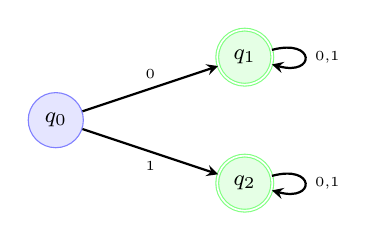
\begin{tikzpicture}[
  state/.style={circle, draw=blue!50, fill=blue!10, minimum size=0.7cm, font=\footnotesize},
  accept/.style={circle, draw=green!50, fill=green!10, minimum size=0.7cm, font=\footnotesize, double},
  arrow/.style={->, >=stealth, thick}
]
  \node[state] (q0) at (0,0) {$q_0$};
  \node[accept] (q1) at (2.4,0.8) {$q_1$};
  \node[accept] (q2) at (2.4,-0.8) {$q_2$};
  \draw[arrow] (q0) -- node[above, font=\tiny] {0} (q1);
  \draw[arrow] (q0) -- node[below, font=\tiny] {1} (q2);
  \draw[arrow] (q1) to[loop right] node[right, font=\tiny] {0,1} (q1);
  \draw[arrow] (q2) to[loop right] node[right, font=\tiny] {0,1} (q2);
\end{tikzpicture}
\caption{DFA non-minimal: $q_1$ dan $q_2$ ekuivalen}
\end{figure}

\subsection{Partisi dan Penggabungan}
\begin{table}[!htbp]
\centering
\begin{tabular}{|l|l|}
\hline
\textbf{Iterasi} & \textbf{Partisi} \\
\hline
$P_0$ & $\{q_1, q_2\}$ (final), $\{q_0\}$ (non-final) \\
\hline
$P_1$ & $\{q_1, q_2\}$, $\{q_0\}$ (tidak berubah) \\
\hline
\end{tabular}
\caption{Refinement partisi untuk contoh DFA}
\end{table}

Karena tidak ada pemisahan lebih lanjut, $q_1$ dan $q_2$ digabung menjadi satu state final.

\section{Implementasi Lexer Hand-written}

Pendekatan \textit{hand-written} memberikan kontrol penuh dan sangat berguna untuk memahami detail proses tokenisasi.

\subsection{Struktur Data Token}
Token minimal harus menyimpan kategori (\textit{type}), string asli (\textit{lexeme}), serta informasi posisi (baris dan kolom) untuk keperluan pelaporan kesalahan.

\begin{lstlisting}[language=C++]
enum class TokenType {
    IDENTIFIER, KEYWORD, INTEGER_LITERAL, FLOAT_LITERAL,
    OP_PLUS, OP_ASSIGN, SEMICOLON, END_OF_FILE, INVALID
};

struct Token {
    TokenType type;
    std::string lexeme;
    int line;
    int column;
};
\end{lstlisting}

\subsection{Arsitektur Kelas Lexer}
Kelas Lexer mengelola input string dan memprosesnya karakter demi karakter menggunakan pointer posisi.

\begin{figure}[!htbp]
    \centering
    \adjustbox{max width=0.8\textwidth,center}{%
    \begin{tikzpicture}[
        class/.style={rectangle, draw=blue!50, fill=blue!10, text width=3cm, minimum height=1cm, font=\footnotesize, align=center, rounded corners},
        method/.style={rectangle, draw=green!50, fill=green!10, text width=2.5cm, minimum height=0.5cm, font=\tiny, align=center},
        arrow/.style={->, >=stealth, thick}
    ]
    \node[class] (lexer) {Lexer Interface};
    \node[method, below=0.6cm of lexer] (p1) {peek() / get()};
    \node[method, right=0.3cm of p1] (p2) {nextToken()};
    \draw[arrow] (lexer) -- (p1);
    \draw[arrow] (lexer) -- (p2);
    \end{tikzpicture}%
    }
    \caption{Komponen utama kelas Lexer}
\end{figure}

\section{Logika State Machine Token}

\subsection{Prinsip Maximal Munch (Longest Match)}
Dalam implementasi lexer, sering terjadi ambiguitas. Misalnya, input \texttt{>=} bisa dibaca sebagai \texttt{>} lalu \texttt{=}, atau sebagai satu token \texttt{>=}. Prinsip standar yang digunakan adalah \textbf{Maximal Munch}: \textit{selalu ambil token terpanjang yang mungkin}.
\begin{itemize}
    \item Jika input adalah \texttt{>=}, lexer akan melihat \texttt{>}. Jangan berhenti! Lihat karakter berikutnya \texttt{=}. Karena \texttt{>=} valid, ambil keduanya.
    \item Jika input adalah \texttt{>a}, lexer melihat \texttt{>}. Karakter berikutnya \texttt{a} tidak membentuk operator valid dengan \texttt{>}. Maka, kembalikan hanya \texttt{>} dan mundurkan kursor dari \texttt{a}.
\end{itemize}

\subsection{Prinsip Prioritas: Keyword vs Identifier}
Pola \texttt{if} cocok dengan aturan \textit{Keyword IF}, tapi juga cocok dengan pola \textit{Identifier}. Bagaimana membedakannya?
\begin{enumerate}
    \item \textbf{Rule Order}: Dalam alat seperti Flex, aturan yang ditulis lebih awal menang. Tulis aturan \texttt{if} sebelum aturan Identifier.
    \item \textbf{Lookup Table}: Dalam lexer manual, kita biasanya menganggap semuanya sebagai Identifier dulu. Setelah lexeme terkumpul ("if"), kita cek ke dalam tabel hash berisi daftar kata kunci. Jika ada, ubah tipe tokennya menjadi \texttt{KW\_IF}. Ini lebih efisien daripada membuat state machine DFA yang sangat kompleks untuk setiap kata kunci.
\end{enumerate}

\begin{figure}[!htbp]
    \centering
    \adjustbox{max width=0.8\textwidth,center}{%
    \begin{tikzpicture}[
        state/.style={circle, draw=blue!50, fill=blue!10, minimum size=0.8cm, font=\tiny, align=center},
        start/.style={circle, draw=red!50, fill=red!10, minimum size=0.8cm, font=\tiny, align=center},
        accept/.style={circle, draw=green!50, fill=green!10, minimum size=0.8cm, font=\tiny, double},
        arrow/.style={->, >=stealth, thick}
    ]
    \node[start] (q0) {START};
    \node[state, right=2cm of q0] (q1) {IN\_ID};
    \node[accept, right=2cm of q1] (q2) {DONE};
    \draw[arrow] (q0) -- node[above, font=\tiny] {letter/\_} (q1);
    \draw[arrow] (q1) to[loop above] node[above, font=\tiny] {alnum/\_} (q1);
    \draw[arrow] (q1) -- node[above, font=\tiny] {other} (q2);
    \node[below=0.5cm of q1, font=\itshape\footnotesize] {Setelah DONE, cek HashMap Keywords};
    \end{tikzpicture}%
    }
    \caption{State machine generik untuk Identifier/Keyword}
\end{figure}

\subsection{State Machine untuk Angka}
Menangani angka juga membutuhkan logika \textit{lookahead}. Saat melihat titik (\texttt{.}), lexer harus memastikan karakter selanjutnya adalah digit sebelum memutuskannya sebagai \texttt{FLOAT\_LITERAL}. Jika tidak (misal \texttt{1..10} di Pascal), titik tersebut mungkin token terpisah (\textit{range operator}).

\begin{lstlisting}[language=C++]
Token Lexer::scanNumber() {
    std::string text;
    while (isdigit(peek())) text += advance();
    
    if (peek() == '.' && isdigit(peekNext())) { // Lookahead 2 langkah
        text += advance(); // makan titik
        while (isdigit(peek())) text += advance();
        return Token(FLOAT, text);
    }
    return Token(INT, text);
}
\end{lstlisting}

\section{Handling Komentar dan Kesalahan}

\subsection{Whitespace dan Pelacakan Posisi}
Kompilator umumnya mengabaikan \textit{whitespace} (spasi, tab, newline) kecuali pada bahasa sensitif-indentasi seperti Python. Namun, whitespace memiliki peran krusial: memperbarui penghitung baris (\texttt{line counter}). Informasi baris ini sangat vital untuk pesan kesalahan nanti.
\begin{lstlisting}[language=C++]
void Lexer::skipWhitespace() {
    while (isspace(peek())) {
        if (peek() == '\n') {
            line++; col = 0; // Reset kolom
        } else {
            col++;
        }
        advance();
    }
}
\end{lstlisting}

\subsection{Penanganan Komentar Bersarang}
Komentar C standar (\texttt{/* ... */}) tidak mendukung \textit{nesting}. Jika parser menemukan \texttt{/* A /* B */ C */}, ia akan berhenti pada \texttt{*/} pertama (setelah B), menyebabkan \texttt{C */} dianggap sebagai kode \textit{syntax error}. Jika ingin mendukung \textit{nested comments} (seperti di Swift), lexer harus menggunakan counter kedalaman.

\subsection{Strategi Pemulihan Kesalahan Leksikal}
Ketika lexer menemukan karakter ilegal (misal: \texttt{@} di C), ia tidak boleh langsung \textit{crash}. Ada beberapa strategi pemulihan:
\begin{itemize}
    \item \textbf{Panic Mode}: Abaikan karakter bermasalah dan coba lanjut memindai karakter berikutnya. Ini strategi paling umum.
    \item \textbf{Error Token}: Kembalikan token khusus \texttt{TK\_ERROR} ke parser, biarkan parser yang memutuskan apakah akan berhenti atau mencoba pulih.
    \item \textbf{Deletion/Insertion}: Mencoba menghapus karakter aneh atau menyisipkan karakter yang hilang (misal: menutup string yang terbuka), tapi ini berisiko mengubah makna program.
\end{itemize}

\begin{figure}[!htbp]
    \centering
    \adjustbox{max width=0.8\textwidth,center}{%
    \begin{tikzpicture}[
        char/.style={rectangle, draw=blue!50, fill=blue!10, minimum width=0.6cm, font=\tiny},
        err/.style={rectangle, draw=red!50, fill=red!10, minimum width=1.5cm, font=\tiny, align=center},
        arrow/.style={->, >=stealth, thick}
    ]
    \node[char] (c1) {"}; \node[char, right=0.2cm of c1] (c2) {h}; \node[char, right=0.2cm of c2] (c3) {e};
    \node[char, right=0.2cm of c3] (c4) {EOF};
    \node[err, below=0.6cm of c4] (msg) {Error: Unclosed String};
    \draw[arrow, red] (c4) -- (msg);
    \end{tikzpicture}%
    }
    \caption{Ilustrasi unclosed string error}
\end{figure}

\section{Lexer Generator dan Best Practices}

\subsection{Penggunaan Flex}
Untuk proyek skala besar, penggunaan generator seperti \textit{Flex} lebih disarankan. Kita cukup menulis pola regex, dan Flex akan men-generate code C/C++ yang sangat efisien secara otomatis.

\subsection{Best Practices}
\begin{enumerate}
    \item \textbf{Lookahead}: Gunakan fungsi \texttt{peek()} untuk mengintip karakter berikutnya tanpa menghabiskannya.
    \item \textbf{Position Tracking}: Simpan baris dan kolom untuk mempermudah \textit{debugging} bagi pemrogram.
    \item \textbf{Longest Match}: Selalu ambil token terpanjang yang cocok (misal: \texttt{==} lebih prioritas daripada \texttt{=}).
\end{enumerate}

\section{Lexer Generator: Flex dan re2c}

Lexer generator adalah alat yang secara otomatis membangun \textit{finite automata} dari spesifikasi ekspresi reguler.

\subsection{Flex (Fast Lexical Analyzer)}
Flex adalah generator standar yang paling luas digunakan. Spesifikasinya ditulis dalam file \texttt{.l} dengan tiga bagian utama: \textit{Definitions}, \textit{Rules}, dan \textit{User Code}.

\begin{figure}[!htbp]
    \centering
    \adjustbox{max width=0.8\textwidth,center}{%
    \begin{tikzpicture}[
        file/.style={rectangle, draw=blue!50, fill=blue!10, text width=2cm, font=\tiny, align=center},
        proc/.style={rectangle, draw=green!50, fill=green!10, text width=2cm, font=\tiny, align=center},
        arrow/.style={->, >=stealth, thick}
    ]
    \node[file] (spec) {lexer.l};
    \node[proc, right=1cm of spec] (flex) {Flex Generator};
    \node[file, right=1cm of flex] (code) {lex.yy.c};
    \draw[arrow] (spec) -- (flex);
    \draw[arrow] (flex) -- (code);
    \end{tikzpicture}%
    }
    \caption{Alur kerja Flex}
\end{figure}

\subsection{re2c}
re2c adalah generator modern yang menghasilkan kode C/C++ berperforma sangat tinggi. Berbeda dengan Flex, re2c menyisipkan spesifikasinya langsung di dalam komentar khusus pada file sumber C/C++.

\subsection{Perbandingan Pendekatan}
\begin{table}[!htbp]
\centering
\begin{tabular}{|l|c|c|c|}
\hline
\textbf{Fitur} & \textbf{Hand-written} & \textbf{Flex} & \textbf{re2c} \\
\hline
Produktivitas & Rendah & Tinggi & Tinggi \\
Performa & Tinggi & Sedang & Sangat Tinggi \\
Maintenance & Sulit & Mudah & Mudah \\
\hline
\end{tabular}
\caption{Perbandingan metode konstruksi lexer}
\end{table}


% ============================================================
% AKTIVITAS PEMBELAJARAN
% ============================================================
\begin{aktivitas}
  \item \textbf{Regex Practice}: Buat regular expression untuk email address, URL, dan phone number.
  \item \textbf{NFA to DFA}: Konversi NFA untuk identifier ke DFA dan gambarkan state diagramnya.
  \item \textbf{Lexer Implementation}: Implementasikan lexer sederhana untuk bahasa dengan 5 token types.
  \item \textbf{Tool Exploration}: Coba Flex atau ANTLR untuk generate lexer dari regex definitions.
  \item \textbf{Performance Analysis}: Bandingkan performance hand-coded vs generated lexer.
\end{aktivitas}

% ============================================================
% LATIHAN DAN REFLEKSI
% ============================================================
\begin{latihan}
  \item Buat regular expression untuk mengenali semua valid identifiers dalam bahasa C!
  \item Gambarkan NFA dan DFA untuk regular expression \code{(a|b)*abb}!
  \item Implementasikan DFA recognizer untuk binary numbers yang habis dibagi 3!
  \item Analisis kelebihan dan kekurangan menggunakan generated lexer!
  \item Desain transition table untuk lexer dengan 10 token types!
  \item \textbf{Refleksi}: Bagian mana dari lexical analysis yang paling sulit dan mengapa?
\end{latihan}

% ============================================================
% ASESMEN
% ============================================================
\begin{asesmen}
\textbf{Instrumen Penilaian untuk Sub-CPMK 2.1-2.2}

\textbf{A. Pilihan Ganda}

\begin{enumerate}
  \item Regular expression \code{a(b|c)*d} mengenali:
  \begin{enumerate}
    \item ad, abd, acd
    \item ad, abd, acd, abcd, acbd
    \item ad, abd, acd, abcd, accd, abccd
    \item Hanya string yang dimulai dengan a dan diakhiri d
  \end{enumerate}
  
  \item Perbedaan utama NFA dan DFA adalah:
  \begin{enumerate}
    \item NFA lebih cepat dari DFA
    \item NFA memiliki epsilon transitions
    \item DFA memiliki lebih banyak states
    \item NFA tidak bisa mengenali regular languages
  \end{enumerate}
  
  \item Tool yang paling umum untuk generate lexer adalah:
  \begin{enumerate}
    \item GCC
    \item Flex
    \item Make
    \item GDB
  \end{enumerate}
\end{enumerate}

\textbf{B. Essay}

\begin{enumerate}
  \item Jelaskan langkah-langkah mengkonversi NFA ke DFA dengan contoh konkret!
  \item Desain dan implementasikan lexer untuk bahasa sederhana dengan minimal 8 token types!
\end{enumerate}

\textbf{Rubrik Penilaian}: Lihat Lampiran A
\end{asesmen}

% ============================================================
% CHECKLIST KOMPETENSI
% ============================================================
\begin{checklist}
  \item Saya dapat membuat regular expression untuk token spesifik bahasa
  \item Saya dapat mengimplementasikan NFA untuk token recognition
  \item Saya dapat mengkonversi NFA ke DFA
  \item Saya dapat mengimplementasikan DFA lexer
  \item Saya memahami perbedaan hand-coded vs generated lexer
  \item Saya dapat menggunakan tools modern untuk lexical analysis
\end{checklist}

% ============================================================
% RANGKUMAN
% ============================================================
\begin{rangkuman}
Bab ini membahas lexical analysis, regular expression, dan finite automata sebagai fondasi untuk implementasi lexer. Mahasiswa belajar membuat regex, mengimplementasikan NFA/DFA, dan memahami trade-off berbagai pendekatan lexer implementation.

\textbf{Poin Kunci:}
\begin{itemize}
  \item Lexical analysis mengubah stream of characters menjadi stream of tokens
  \item Regular expression adalah notasi powerful untuk mendeskripsikan token patterns
  \item NFA mudah dibuat tapi DFA lebih efisien untuk execution
  \item Generated lexer (Flex) lebih maintainable, hand-coded lebih optimal
  \item Table-driven lexer adalah pendekatan yang balance antara performance dan maintainability
\end{itemize}

\textbf{Kata Kunci}: \compiler{Lexical Analysis}, \compiler{Regular Expression}, \compiler{NFA}, \compiler{DFA}, \compiler{Token}, \compiler{Lexeme}, \compiler{Flex}, \compiler{Table-Driven Lexer}
\end{rangkuman}

\ifSubfilesClassLoaded{%
    \clearpage
    \printbibliography[title={Daftar Pustaka}]
    \end{refsection}
}{}

\end{document}
